% Problem 2 publication-figure snippets (A-route Final canonical 数据)。
% 时间口径统一 H-END：slot 1 = 0:00-0:10 … slot 144 = 23:50-24:00，横轴为物理时刻 0-24 h。
% 正文图：P2-1 ~ P2-5；补充图：P2-S1 ~ P2-S3；技术路线图：fig_roadmap。

% ---- 正文图 ----
\begin{figure}[htbp]
  \centering
  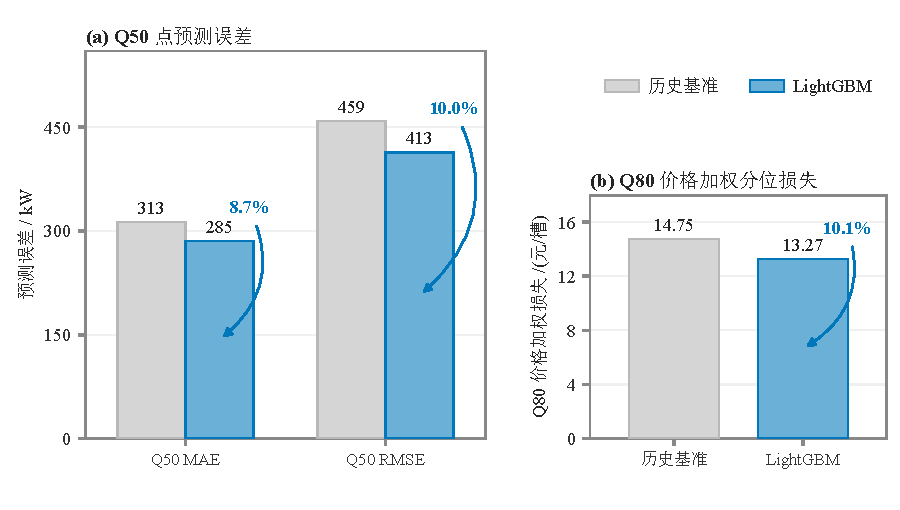
\includegraphics[width=0.85\textwidth]{figures/fig_p2_forecast_metrics.pdf}
  \caption{共同 330 天因果评价区间内历史周期基准与 LightGBM 的预测误差比较。(a) Q50 MAE 与 RMSE 分别由 312.56、459.04 kW 降至 285.26、413.20 kW；(b) Q80 价格加权分位损失由 14.75 元/槽降至 13.27 元/槽（下降 10.1\%）。Q80 经验覆盖率未提高（77.96\%$\to$77.58\%），故仅作描述性误差下降，不宣称全指标占优。数据源：\texttt{data/p2\_forecast\_fair330\_summary.csv}。}
  \label{fig:p2-forecast-metrics}
\end{figure}

\begin{figure}[htbp]
  \centering
  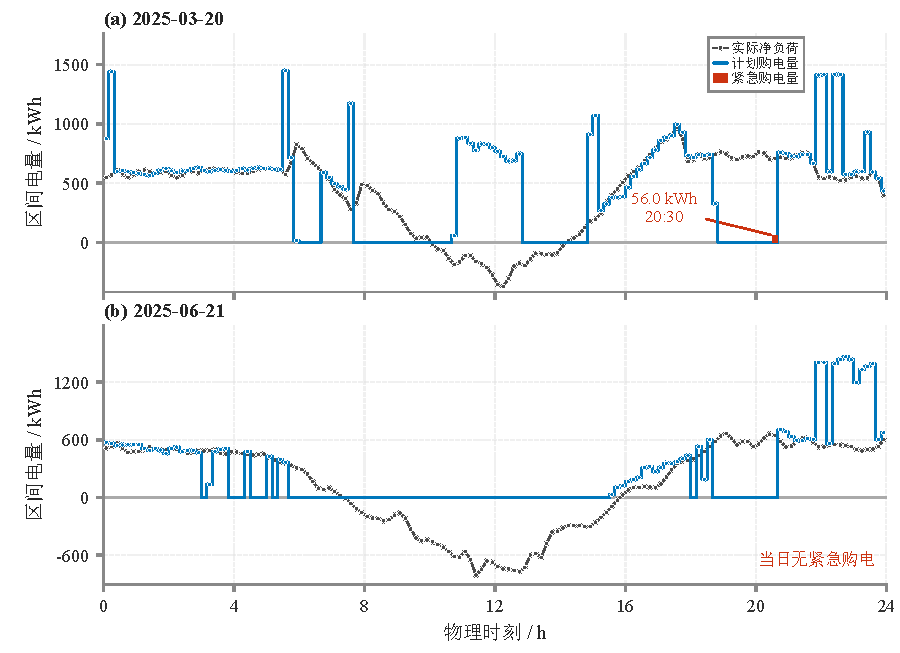
\includegraphics[width=0.85\textwidth]{figures/fig_p2_dispatch_2days.pdf}
  \caption{典型日实际净负荷与购电调度（每 10 min 区间电量）。(a) 2025-03-20 在 20:30--20:40 出现 55.97 kWh 紧急购电；(b) 2025-06-21 无紧急购电，作为对照。计划购电在 0:00 后冻结，储能仅依据当前实际负荷/光伏与当前 SOC 反馈。数据源：\texttt{data/p2\_specified\_dates\_timeseries.csv}。}
  \label{fig:p2-dispatch-2days}
\end{figure}

\begin{figure}[htbp]
  \centering
  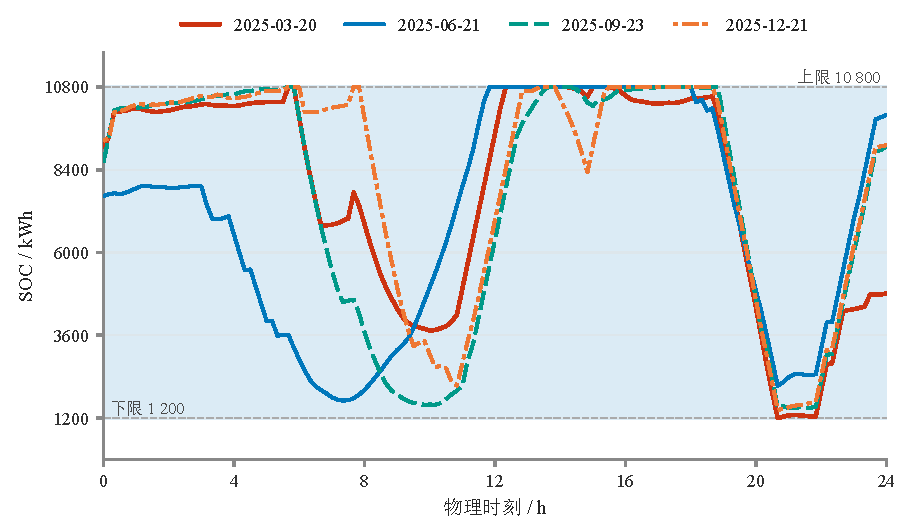
\includegraphics[width=0.85\textwidth]{figures/fig_p2_soc_4days.pdf}
  \caption{四个题目指定日的储能 SOC 轨迹，虚线为 1\,200 / 10\,800 kWh 安全边界。各日 0:00 的 SOC 由前一日结转（不为 6\,000），2025-03-20 触及下限、各日均达上限，表明储能调度受边界约束主导。数据源：\texttt{data/p2\_specified\_dates\_timeseries.csv}。}
  \label{fig:p2-soc-4days}
\end{figure}

\begin{figure}[htbp]
  \centering
  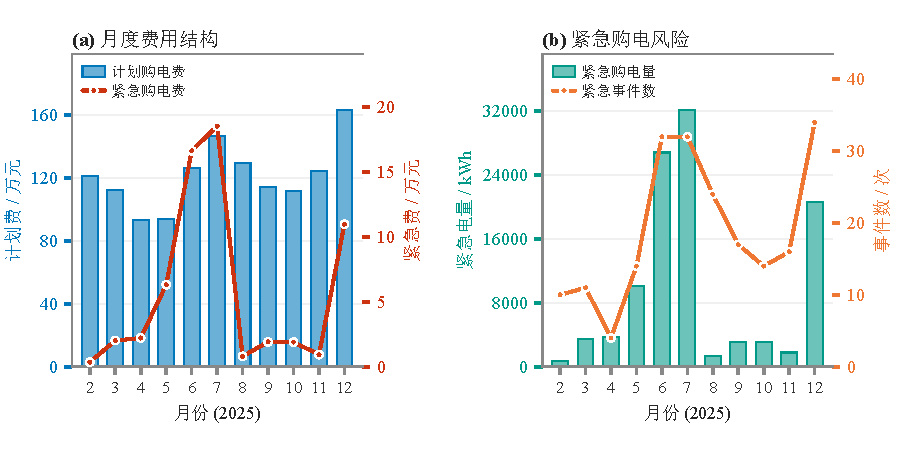
\includegraphics[width=0.85\textwidth]{figures/fig_p2_monthly_cost.pdf}
  \caption{2025 年 2--12 月购电费用结构与紧急购电风险。(a) 蓝柱为月度计划购电费（左轴），红折线为月度紧急购电费（右轴），紧急费在 6--7 月约占当月 11\%、其余月份多在 2\% 以下；(b) 红柱为月度紧急购电量（7 月峰值 32\,064 kWh），青线为月度紧急事件数（12 月 34 次）。全年计划费 13\,350\,598 元、紧急费 626\,125 元。数据源：\texttt{data/p2\_monthly\_cost\_summary\_MAIN.csv}。}
  \label{fig:p2-monthly-cost}
\end{figure}

\begin{figure}[htbp]
  \centering
  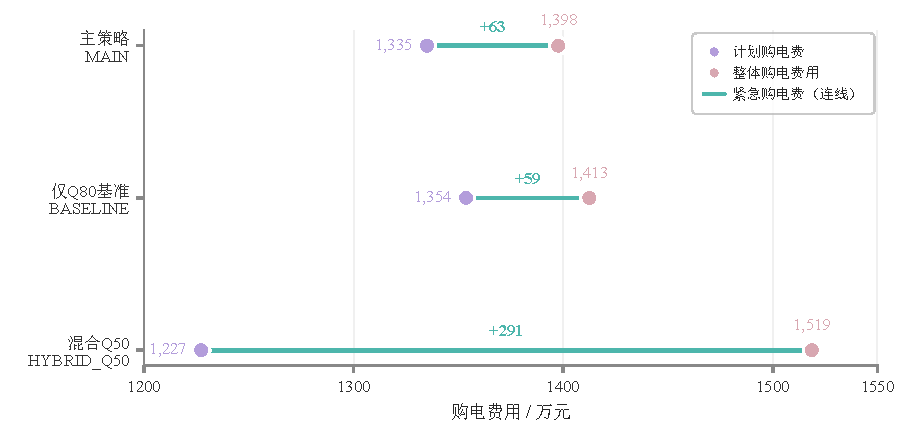
\includegraphics[width=0.85\textwidth]{figures/fig_p2_policy_ablation.pdf}
  \caption{A-5 风险策略消融的费用分解。(a) 主策略 MAIN 总费用 13\,976\,723 元最低；(b) HYBRID\_Q50 虽计划费最低，但 5 倍电价下紧急费高达 291 万元，总费用升至 15\,186\,373 元。MAIN 的优势来自总账而非紧急费最少。数据源：\texttt{data/p2\_policy\_comparison\_A5.csv}。}
  \label{fig:p2-policy-ablation}
\end{figure}

% ---- 补充图 ----
\begin{figure}[htbp]
  \centering
  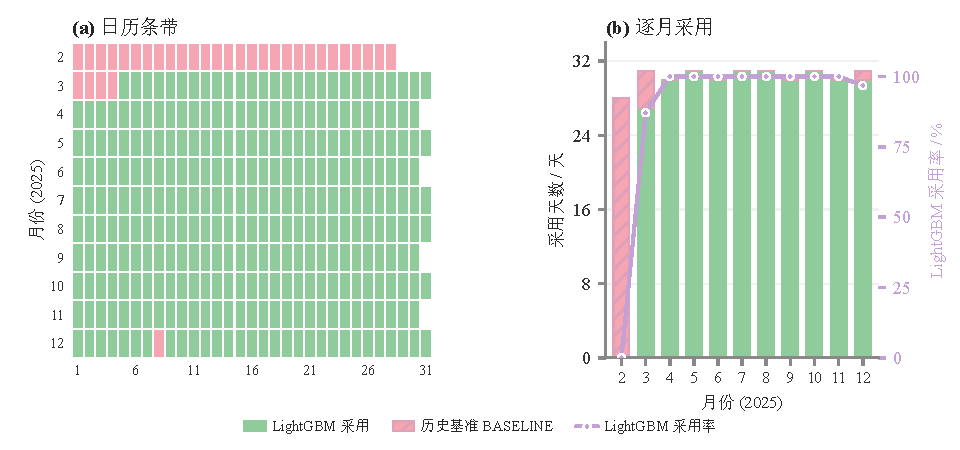
\includegraphics[width=0.85\textwidth]{figures/fig_p2_selector_ratio.pdf}
  \caption{在线 selector 的分支采用情况。(a) 日历条带：每格为一天，薄荷绿=选用 LightGBM、粉=退回历史基准；(b) 逐月采用天数（堆叠柱，橙色段带斜线网格）与月度 LightGBM 采用率（折线）。正式 334 天中 LightGBM 采用 301 天（90.1\%）：2 月整月使用历史基准（因果 warm-up），3 月起切换，12 月仅回退 1 天，说明并非全年强制 LightGBM。数据源：\texttt{data/p2\_selector\_daily.csv}。}
  \label{fig:p2-selector-ratio}
\end{figure}

\begin{figure}[htbp]
  \centering
  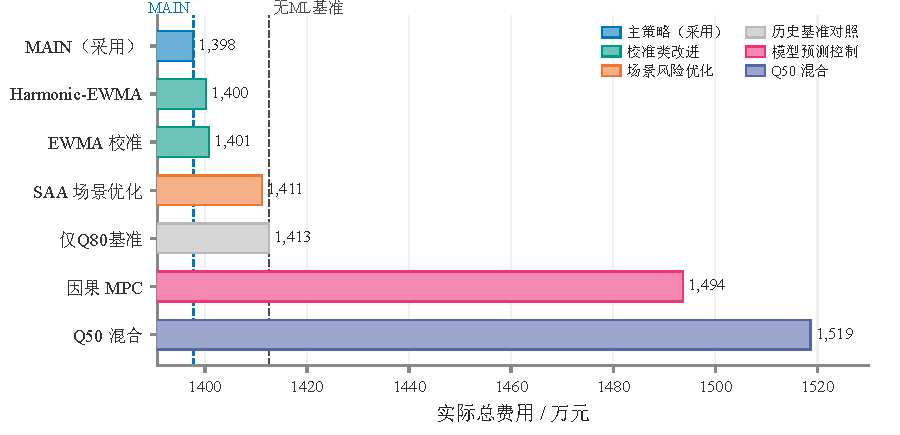
\includegraphics[width=0.85\textwidth]{figures/fig_p2_refinement_compare.pdf}
  \caption{定向改进实验与主策略的总费用对比。SAA、EWMA、Harmonic-EWMA、Causal MPC 等预设方向均未击败 MAIN，说明最终方案经过多方向尝试后保留。数据源：\texttt{data/p2\_experiment\_comparison\_final.csv}。}
  \label{fig:p2-refinement-compare}
\end{figure}

\begin{figure}[htbp]
  \centering
  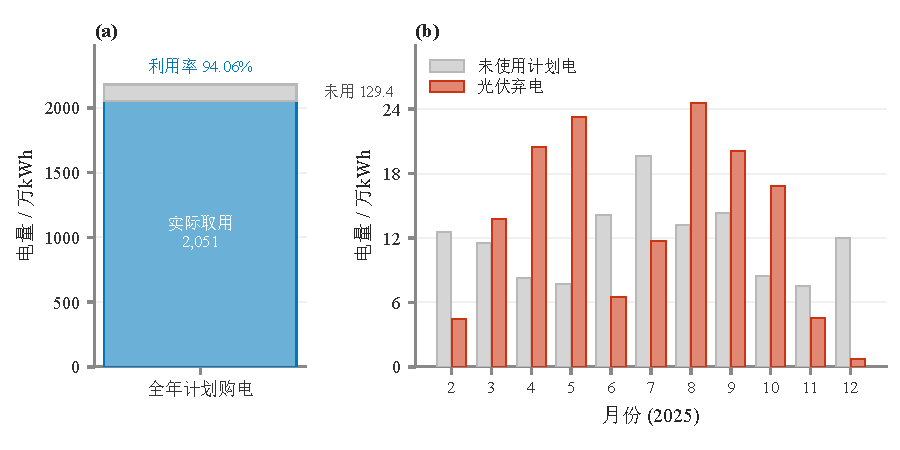
\includegraphics[width=0.85\textwidth]{figures/fig_p2_unused_curtailment.pdf}
  \caption{未使用计划电与光伏弃电诊断。(a) 计划购电利用率 94.06\%（21\,803\,695 kWh 中未用 1\,294\,262 kWh）；(b) 逐月未使用计划电与光伏弃电（全年 1\,469\,771 kWh）是不同概念，不合并为“弃电”。数据源：\texttt{data/p2\_monthly\_cost\_summary\_MAIN.csv}。}
  \label{fig:p2-unused-curtailment}
\end{figure}

% ---- 技术路线图 ----
\begin{figure}[htbp]
  \centering
  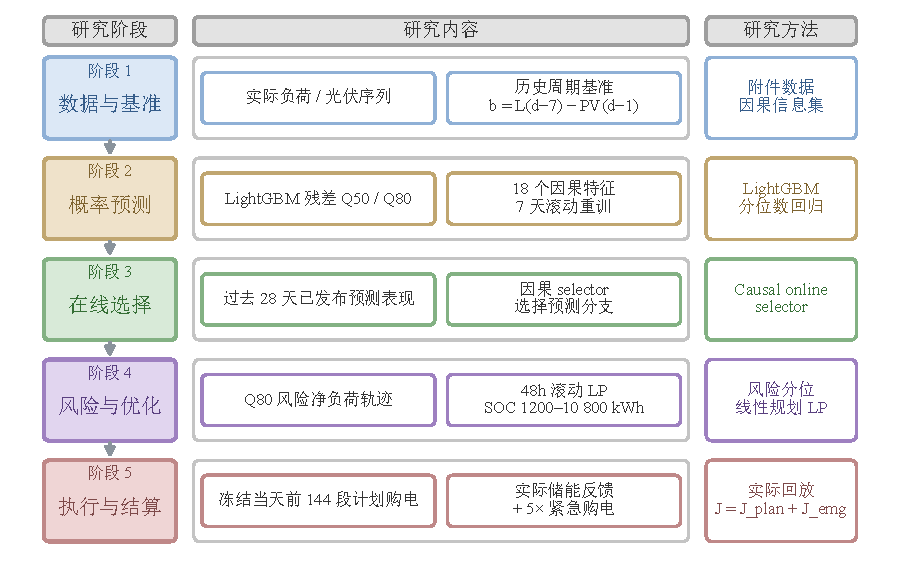
\includegraphics[width=0.9\textwidth,height=0.72\textheight,keepaspectratio]{figures/fig_roadmap.pdf}
  \caption{Problem 2 整体技术路线图。}
  \label{fig:p2-roadmap}
\end{figure}
